% TO-DO:
% * slides to mention big achievements, 附件

\documentclass[10pt]{beamer}
% \geometry{papersize={5in,4.5in}}

\ifdefined\chinchin
\usepackage[CJKspace]{xeCJK}
%\setCJKmainfont[BoldFont=SimHei,ItalicFont=AR PL KaitiM GB]{Alibaba PuHuiTi}
\setCJKmainfont{Alibaba PuHuiTi}
\newcommand{\cc}[2]{#1}
\else
\newcommand{\cc}[2]{#2}
% \renewcommand{\baselinestretch}{0.8}
\fi

%\usepackage{newtxtext,newtxmath}	% use Times Roman font
%\usepackage{newtxtext}
%\renewcommand{\familydefault}{\sfdefault}
\usefonttheme{serif}
\usefonttheme{professionalfonts}
%\setbeamertemplate{theorems}[numbered]
\setbeamertemplate{caption}{\insertcaption} 	% no `Figure' prefix before caption

\mode<presentation> {

%\usetheme{default}
%\usetheme{AnnArbor}
%\usetheme{Antibes}
%\usetheme{Bergen}
%\usetheme{Berkeley}
%\usetheme{Berlin}
%\usetheme{Boadilla}
%\usetheme{CambridgeUS}
%\usetheme{Copenhagen}
%\usetheme{Darmstadt}
%\usetheme{Dresden}
%\usetheme{Frankfurt}
%\usetheme{Goettingen}
%\usetheme{Hannover}
%\usetheme{Ilmenau}
%\usetheme{JuanLesPins}
%\usetheme{Luebeck}
\usetheme{Madrid}
%\usetheme{Malmoe}
%\usetheme{Marburg}
%\usetheme{Montpellier}
%\usetheme{PaloAlto}
%\usetheme{Pittsburgh}
%\usetheme{Rochester}
%\usetheme{Singapore}
%\usetheme{Szeged}
%\usetheme{Warsaw}

%\usecolortheme{albatross}
%\usecolortheme{beaver}
%\usecolortheme{beetle}
%\usecolortheme{crane}
%\usecolortheme{dolphin}
%\usecolortheme{dove}
%\usecolortheme{fly}
%\usecolortheme{lily}
\usecolortheme{orchid}
%\usecolortheme{rose}
%\usecolortheme{seagull}
%\usecolortheme{seahorse}
%\usecolortheme{whale}
%\usecolortheme{wolverine}		% Hofstra

%\setbeamertemplate{footline} % To remove the footer line in all slides uncomment this line
\setbeamertemplate{footline}[page number] % To replace the footer line in all slides with a simple slide count uncomment this line
\setbeamertemplate{navigation symbols}{} % To remove the navigation symbols from the bottom of all slides uncomment this line
}

\setbeamertemplate{headline}{}
% \setbeamersize{text margin left=1mm,text margin right=1mm}
% \settowidth{\leftmargini}{\usebeamertemplate{itemize item}}
% \addtolength{\leftmargini}{\labelsep}
% \setbeamertemplate{enumerate subitem}{(\roman{enumii})}
% \setbeamertemplate{itemize items}[default]
\setbeamertemplate{items}[square]
\setbeamertemplate{enumerate items}[default]

\usepackage[backend=biber,style=numeric]{biblatex}
\bibliography{../../AGI-book}
% \renewcommand*{\bibfont}{\footnotesize}
\setbeamertemplate{bibliography item}[text]

\usepackage{graphicx} % Allows including images
\usepackage{tikz-cd}
\usetikzlibrary{decorations.pathmorphing}
% \usepackage{tikz}
\usepackage[export]{adjustbox}% http://ctan.org/pkg/adjustbox
\usepackage{verbatim} % comments
\usepackage[skins,theorems]{tcolorbox}

\usepackage{ulem}
\makeatletter
\newcommand{\cthickuline}[3][0.5pt]{%
	\UL@protected\def\temp@uline{\bgroup\markoverwith
		{\textcolor{#2}{\rule[-0.5ex]{2pt}{#1}}}\ULon}%
	\temp@uline{#3}%
}
\makeatother

% \usepackage{tikz-cd}  % commutative diagrams
% \newcommand{\tikzmark}[1]{\tikz[overlay,remember picture] \node (#1) {};}
% \usepackage{booktabs} % Allows the use of \toprule, \midrule and \bottomrule in tables
% \usepackage{amssymb}  % \leftrightharpoons
% \usepackage{wasysym} % frownie face
% \usepackage{newtxtext,newtxmath}	% Times New Roman font
% \usepackage{sansmath}

\let\oldtextbf\textbf
\renewcommand{\textbf}[1]{\textcolor{blue}{\oldtextbf{#1}}}
\newcommand{\emp}[1]{\textbf{\color{violet}#1}}

\newcommand{\vect}[1]{\boldsymbol{#1}}
\newcommand{\tab}{\hspace*{1cm}}
\newcommand*\confoundFace{$\vcenter{\hbox{\includegraphics[scale=0.2]{../../confounded-face.jpg}}}$}
\newcommand{\smiley}{$\vcenter{\hbox{\includegraphics[scale=0.05]{../../smiling-face.png}}}$}
\newcommand{\cubic}{\vcenter{\hbox{\includegraphics[scale=1]{../../cubic-symbol.png}}}}

\makeatletter
\renewcommand{\boxed}[1]{\fbox{\m@th$\displaystyle\scalebox{0.9}{#1}$} \,}
\makeatother

%----------------------------------------------------------------------------------------
%	TITLE PAGE
%----------------------------------------------------------------------------------------

\title[AGI and categorical logic]{{Paper: Combining RL, LLM, and Logic}}
\author{\includegraphics[scale=0.14]{John_Grothendieck.png} \\ \centering YKY}
\date{\today} % Date, can be changed to a custom date

\begin{document}

\addtocounter{page}{-1}
\begin{frame}[plain,noframenumbering]
\titlepage
\end{frame}

\addtocounter{page}{-1}
\begin{frame}[noframenumbering]
\frametitle{Contents}
\fontsize{10pt}{8}\selectfont

\end{frame}

%----------------------------------------------------------------------------------------
%	PRESENTATION SLIDES
%----------------------------------------------------------------------------------------

\part{GPT envy}
\frame{\partpage}

\begin{frame}
\frametitle{AGI as graph rewriting}

\begin{itemize}
	\item Ben Goertzel in his \textit{General Theory of General Intelligence} posits AGI as a [hyper- or meta-] graph-rewriting system.

	\item YKY proposes a similar but less general architecture where Working Memory = tree, and inference = tree-rewriting a.k.a. term-rewriting.
	\begin{equation}
		\vcenter{\hbox{\includegraphics[scale=0.5]{tree-rewriting.png}}}
		\nonumber
	\end{equation}

	\item YKY further proposes a \textbf{differentiable} version of the rewriting rules, and compares them with the traditional Transformer.

	\item Abstract rewriting can be formulated categorically as morphisms satisfying certain commutative relations.  This is an \textbf{algebraic} way of formalizing intelligence, using \textbf{discrete} data structures.
\end{itemize}
\end{frame}

\begin{frame}
\frametitle{String-diagram Kung-fu}

\begin{itemize}
	\item This is a string diagram of Self-Attention:
	\begin{equation}
		\vcenter{\hbox{\includegraphics[scale=0.5]{Attention-string-diagram.png}}}
		\nonumber
	\end{equation}

	\item It is possible to ``morph'' string diagrams via string-rewriting.

	\item Some researchers proposed \textbf{universal approximation} as an equivalence class of functions under string-rewriting.  But such a class is too permissive and pretty useless.

	\item We need more \textit{refined} string-rewriting so that we can distinguish between architectures that are more \textbf{learning-efficient} than others.

	\item One source of \textbf{inequivalence} is that functions like sigmoid and softmax can irreversibly ``tear'' the input space into disconnected regions due to finite precision.  This gives rise to ``\textbf{discretizing}'' operations such as the ability of Transformers to output discrete tokens.
\end{itemize}
\end{frame}

\begin{frame}
\frametitle{Counting computations}

\begin{itemize}
	\item In order to answer the ultimate question ``how to design more efficient AGI architectures'', we need to \textbf{count the number of computations} in each morphism.

	\item We start with a Working Memory representation that we are familiar with -- I suggest a tree or forest of trees -- and with a set of reasonably versatile rewriting rules as morphisms.

	\item Develop a set of ``string-fu'' skills to ``functor'' from one architecture to another, while 1) keeping track of discretizing operations, and 2) counting computations; till we end up with a category with the most efficient morphisms.
\end{itemize}
\end{frame}


\part{Logic Transformer}
\frame{\partpage}

\begin{frame}
\frametitle{Curry-Howard isomorphism}
\end{frame}

\begin{frame}
\frametitle{References}
\cc{多谢收看}{Thanks for watching} \smiley \vspace{1cm}
\printbibliography
\end{frame}

\end{document}